% Decision Models as Universal Tool Selectors (paper v2).
% Self-contained: compile with `latexmk -pdf dm_tool_selectors.tex` in this folder.
% Figures: make_figures.py (reads the run records); analysis plans: plans/*.md, included verbatim in Appendix C.
\documentclass[11pt]{article}
\usepackage[T1]{fontenc}
\usepackage[utf8]{inputenc}
\usepackage{lmodern}
\usepackage{microtype}
\usepackage[margin=1in]{geometry}
\usepackage{amsmath,amssymb}
\usepackage{booktabs}
\usepackage{tabularx}
\usepackage{multirow}
\usepackage{graphicx}
\usepackage{xcolor}
\usepackage{enumitem}
\usepackage{caption}
\usepackage{fvextra}
\usepackage{longtable}
\usepackage{array}
\usepackage{tikz}
\usetikzlibrary{positioning,arrows.meta,fit,calc}
\usepackage[numbers,sort&compress]{natbib}
\usepackage{xurl}
\usepackage[colorlinks=true,linkcolor=blue!50!black,citecolor=blue!50!black,urlcolor=blue!50!black]{hyperref}

\setlist{itemsep=2pt,topsep=3pt}
\captionsetup{font=small,labelfont=bf}
\setlength{\emergencystretch}{3em}
\let\oldus\_\renewcommand{\_}{\oldus\discretionary{}{}{}}
\newcommand{\msd}{Microsoft Decision~1}
\newcommand{\F}{selector~F}

\title{\textbf{Decision Models as Universal Tool Selectors}}
\author{Aziz Muminov \and Alexandra Ilina}
\date{November 2026}

\begin{document}
\maketitle

\begin{abstract}
Agents increasingly work through many tools: a coding agent connected to a company's MCP servers can face hundreds
or thousands of tool definitions. Loading them all is expensive: for 613 tools the largest prompt reached about 182k
tokens and a run cost 8--9 times as much as with search. Shipped harnesses therefore search instead, mostly with BM25,
as in Codex, Anthropic's tool search and Hermes Agent. Lexical search is cheap but imprecise, and every extra search
is a full agent turn. We propose decision models, which return a probability per option in one forward pass, as
general-purpose tool selectors. Our selector, built on \msd{}, chooses the service, then the tools, with a ``none''
option and usage-based recommendations, and needs about three decision-model calls per search. On the real tool
definitions of 30 MCP servers with 1{,}076 tools it ranks far better than BM25 offline, with the right tool first for
92\% of hand-written queries against 49\%. Inside a shipped agent, Hermes Agent, on 37 coding tasks with simulated
back ends, pre-planned paired tests run at the same time showed 12.6\% fewer tokens with DeepSeek V4.1 Flash over 555
pairs, $p=0.0002$, and 9.7\% fewer with GPT-6.1 Sol over 185 pairs, $p=0.004$, with 36--60\% fewer searches and equal
pass rates. The selector's fee made runs 20\% more expensive with the inexpensive model and left cost unchanged with
the frontier model; savings grow with the agent model's price and with how much it searches. These results cover
coding agents, simulated services, two agent models and one harness for the main tests.
\end{abstract}

%=====================================================================
\section{Introduction}\label{sec:intro}
%=====================================================================
Through the Model Context Protocol, MCP~\citep{mcp}, an agent can read CI logs, error trackers, tickets, chat,
dashboards, clusters and databases. Each server exposes tens to hundreds of tools, and agents connect to many
servers, so which tools the agent sees, and how it finds the rest, now shapes cost and behaviour.

There are two options. The first is to load every definition into every request. For the 613 tools of twelve
popular servers the largest prompt then reaches about 182k tokens, against 12--16k with search, and a run costs 8--9
times as much at the same pass rate (\S\ref{sec:opencode}). The second, which harnesses ship, is search: definitions
stay out of the prompt and the agent finds tools on demand (Table~\ref{tab:mechanisms}). Most shipped search is
BM25~\citep{codexcli,anthropic2025toolsearch,hermesagent}. BM25 is cheap and needs no model, but it is imprecise, so
agents search repeatedly, and each search is a full LLM turn that re-reads the whole context. With a frontier agent
model, a wasted search costs far more than the search itself.

\emph{Decision models}, or DMs, read a state and a question with named options and return a probability per option
in one forward pass, without generating text. They are cheap and fast, and choosing among named options is what tool
selection asks for. Our thesis is that a DM can serve as a drop-in, harness-agnostic tool selector: one API call per
search, no training, and no change to the agent. We test it with \msd{}~\citep{msd1}.

\paragraph{Contributions.}
\begin{itemize}
\item A DM tool selector, \F{}, and the analyses behind its design: choose services first with a ``none'' option,
then ask two questions per service, and fill a fixed-size answer with usage-based names (\S\ref{sec:selector},
\S\ref{sec:study}).
\item A test suite built on the real tool definitions of 30 MCP servers, with simulated back ends, 38 graded coding
tasks and isolated agent runs (\S\ref{sec:setup}).
\item A protocol for measuring token differences between agent configurations: same-time pairs, task-level
analysis, power planning and written analysis plans with logged interim looks (\S\ref{sec:measuring}).
\item Results for two agent models in Hermes Agent: \F{} used 12.6\% fewer tokens than BM25 with DeepSeek V4.1 Flash
and 9.7\% fewer with GPT-6.1 Sol, at equal pass rates (\S\ref{sec:main}, \S\ref{sec:sol}).
\end{itemize}
The scope is limited: coding agents, simulated services, two agent models and one harness for the main tests
(\S\ref{sec:threats}). ``Universal'' names the proposal, a selector that needs nothing from the harness but a
query, not a result we have shown for every setting.

%=====================================================================
\section{Background: how harnesses select tools, and decision models}\label{sec:background}
%=====================================================================
Table~\ref{tab:mechanisms} lists the mechanisms harnesses ship and the conditions we use to reproduce them. All but
native loading give the agent a search tool and a way to call what it finds, usually with a short overview of the
connected servers, so the agent pays for a definition only when it retrieves it.

\begin{table}[t]
\centering\footnotesize
\caption{Tool-selection mechanisms and the conditions that reproduce them. Used in: M, main tests in Hermes Agent,
\S\ref{sec:main}--\S\ref{sec:sol}; R, offline retrieval, \S\ref{sec:retrieval}; O, opencode, \S\ref{sec:opencode};
E, the earlier six-ranker run, App.~\ref{app:sixrank}.}
\label{tab:mechanisms}
\setlength{\tabcolsep}{4pt}
\begin{tabularx}{\linewidth}{@{}l >{\raggedright\arraybackslash}p{3.7cm} X l@{}}
\toprule
Condition & Shipped or proposed in & What the agent sees and does & Used in \\
\midrule
native & Cursor, Cline, opencode; Claude Code with search off & every tool definition in every request & O \\
cc & Claude Code ToolSearch~\citep{claudecode} & names of all deferred tools; selection by exact name or keyword search weighted towards names; our approximation, since the exact scoring is undocumented & R O E \\
bm25 & Anthropic tool search~\citep{anthropic2025toolsearch}, Codex CLI~\citep{codexcli}, Hermes Agent~\citep{hermesagent} & Okapi BM25~\citep{robertson2009bm25} over names, descriptions and parameters & M R O E \\
groups & GitHub Copilot virtual tools~\citep{copilotvirtualtools} & one activation tool per server group; activating loads the group's definitions & O \\
embed & RAG-MCP~\citep{gan2025ragmcp}; Goose in 2025, since removed~\citep{goose} & cosine similarity of query and tool embeddings & R O E \\
llm & Goose in 2025, since removed~\citep{goose}; AnyTool-style routing~\citep{du2024anytool} & an LLM reads one line per tool and names the best ones & R O \\
dm & this paper, first version & \msd{} ranks servers, then tools & R O E \\
\F{} & this paper & \msd{} chooses services with a ``none'' option, then tools; five tools with descriptions plus names, \S\ref{sec:selector} & M \\
\bottomrule
\end{tabularx}
\end{table}

\paragraph{Hermes Agent's bridge.} Hermes Agent 0.19.0 defers MCP tools once their definitions exceed 10\% of the
context window, as hundreds of tools do. Its \texttt{tool\_search} returns compact hits, a name and one line each;
\texttt{tool\_describe} returns one full definition; found tools are then called directly with typed arguments. Only
the ranker behind \texttt{tool\_search} differs between our main conditions.

\paragraph{Decision models.} A request to OpenRouter's Decisions API~\citep{openrouterdecisions} carries a
\emph{state}, here the agent's search query, and one or more named questions. A multiple-choice question lists up to
255 options, each with a free-text description, and returns a probability per option; a yes/no question returns one
probability. \msd{} is post-trained from Qwen3.5-9B~\citep{msd1} and costs about \$0.04 per million input tokens. We
also benchmarked TypeSafe Jev~\citep{typesafejev} offline at 1{,}076 tools: both put the right tool first for 87.5\%
of queries and in the top five for 95.8\%; Jev answered twice as fast, a median of 0.27 against 0.57\,s, but cost
\$0.211 against \$0.145 per 1{,}000 searches and wrongly answered ``none'' for 1.7\% of queries against 0\%. We use
\msd{} throughout.

%=====================================================================
\section{The DM tool selector}\label{sec:selector}
%=====================================================================
Selector~F answers each \texttt{tool\_search} query in two rounds of DM calls (Figure~\ref{fig:flow}).

\paragraph{Service step.} One multiple-choice question, ``Which service has the tool the agent needs?'', lists a
card for each of the 30 services and a ``none'' option. If $P(\text{none})\ge 0.4$ the answer is empty. Otherwise
the selector takes services in order of probability until they cover 90\% of the probability, at most three, and
always includes a service that the query names. Card quality matters: the original cards confused GitHub, Git and
GitLab, and the fixed cards say that GitHub hosts branches, commits and files, that Git is only the local working copy,
and that GitLab hosts legacy projects (\S\ref{sec:failures}).

\paragraph{Tool step.} For each chosen service, in parallel, two multiple-choice questions over its tools, each tool
described by its name, the start of its description and its parameter names: ``Which tool best serves what the agent
wants to do?'' and ``Which tool would an expert engineer call first to do what the agent wants?''. Scores are
weighted by the service probability. The answer holds the five tools that best serve the query, with Hermes's
one-line descriptions, and then, as names only, up to three prerequisites from the second question and the chosen
services' most-used tools, at most 15 tools in all. Tools already shown in the run are not repeated. The usage lists
are built leave-one-task-out from an earlier run, so a task never sees usage from its own runs.

\paragraph{Why this shape.} Agents work service by service and use three to four tools per service, most of them in
later steps; descriptions are expensive and names are cheap; and the DM's probabilities are too peaked to size a list,
so the list size is fixed and filled by prerequisites and usage. The offline study of \S\ref{sec:study} chose each
element.

\paragraph{Cost.} A search takes about three DM calls in two sequential rounds. In the main tests a search took a
median of 1.0\,s and cost \$0.36 per 1{,}000 searches; 5.7\% of searches got the empty ``none'' answer.

\begin{figure}[t]
\centering
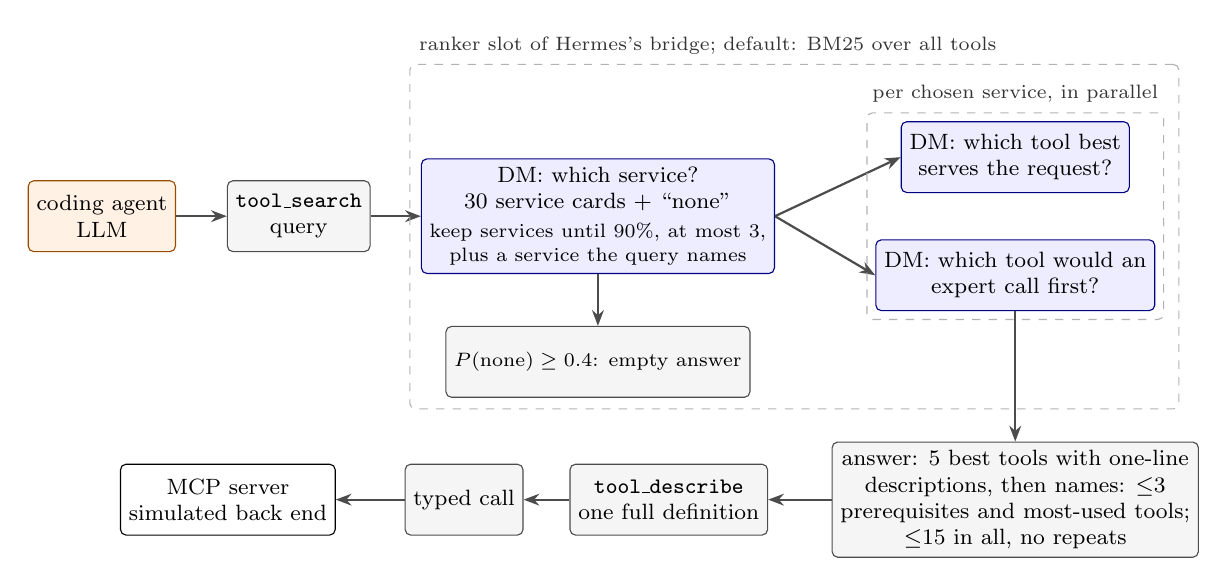
\begin{tikzpicture}[font=\footnotesize,
  box/.style={draw, rounded corners=2pt, align=center, inner sep=3pt, minimum height=9mm, fill=white},
  dm/.style={box, fill=blue!7, draw=blue!50!black}, llm/.style={box, fill=orange!10, draw=orange!60!black},
  outb/.style={box, fill=gray!8, draw=gray!60!black}, arr/.style={-{Stealth[length=2mm]}, thick, draw=gray!60!black}]
\node[llm] (agent) at (0,0) {coding agent\\LLM};
\node[outb] (search) at (2.5,0) {\texttt{tool\_search}\\query};
\node[dm] (srv) at (6.3,0) {DM: which service?\\30 service cards + ``none''\\[1pt]
  {\scriptsize keep services until 90\%, at most 3,}\\[-1pt] {\scriptsize plus a service the query names}};
\node[dm] (best) at (11.6,0.75) {DM: which tool best\\serves the request?};
\node[dm] (first) at (11.6,-0.75) {DM: which tool would an\\expert call first?};
\node[outb, font=\scriptsize] (none) at (6.3,-1.85) {$P(\text{none})\ge0.4$: empty answer};
\node[outb] (ans) at (11.6,-3.6) {answer: 5 best tools with one-line\\descriptions, then names: $\le$3\\prerequisites and most-used tools;\\$\le$15 in all, no repeats};
\node[outb] (desc) at (7.2,-3.6) {\texttt{tool\_describe}\\one full definition};
\node[outb] (call) at (4.6,-3.6) {typed call};
\node[box] (svc) at (1.6,-3.6) {MCP server\\simulated back end};
\draw[arr] (agent) -- (search);
\draw[arr] (search) -- (srv);
\draw[arr] (srv.east) -- (best.west);
\draw[arr] (srv.east) -- (first.west);
\draw[arr] (srv) -- (none);
\draw[arr] (first) -- (ans);
\draw[arr] (ans) -- (desc);
\draw[arr] (desc) -- (call);
\draw[arr] (call) -- (svc);
\node[draw=gray!60, dashed, rounded corners=2pt, fit=(best)(first), inner sep=3pt] (par) {};
\node[font=\scriptsize, text=gray!40!black, anchor=south] (parlab) at (par.north) {per chosen service, in parallel};
\node[draw=gray!60, dashed, rounded corners=2pt, fit=(srv)(par)(parlab)(none), inner sep=4pt] (slot) {};
\node[font=\scriptsize, text=gray!40!black, anchor=south west] at (slot.north west) {ranker slot of Hermes's bridge; default: BM25 over all tools};
\end{tikzpicture}
\caption{Selector~F inside Hermes Agent's search bridge. The agent's query goes to the ranker slot. One DM call chooses the
services or answers ``none''; then two DM calls per chosen service run in parallel. The agent receives five compact
hits and a list of names, reads full definitions with \texttt{tool\_describe} and calls tools directly. In the
baseline, BM25 fills the same slot; everything outside the slot is identical.}
\label{fig:flow}
\end{figure}

%=====================================================================
\section{Experimental setup}\label{sec:setup}
%=====================================================================
\paragraph{Tool catalog.} We started each MCP server as an unprivileged user with dummy credentials and saved its
\texttt{tools/list} response: names, descriptions and input schemas exactly as published. No tool was ever executed
against a real service. The main catalog has 613 tools from 12 popular servers; 18 further servers bring it to
1{,}076 tools, including decoys such as GitLab beside GitHub, AWS CloudWatch beside Grafana and AWS EKS beside
Kubernetes. App.~\ref{app:catalog} lists all servers.

\paragraph{Simulated back ends.} Each task has a world of rules that map a tool and matching argument values to a
response, followed by organisation-wide facts shared by all tasks. Unmatched reads return an empty list or ``not
found''; unmatched writes succeed and are recorded for grading. Arguments are validated against the tool's schema.

\paragraph{Tasks.} Each task is a small Python repository whose fix needs information that exists only in the
services, such as a failing CI check, a Sentry stack trace or a decision in Slack. Task set v2 has 38
\emph{symptom-first} tasks that do not name the service: 23 single-service, 7 multi-service, 4 \emph{absent}, where
the information does not exist and the right outcome is to stop and leave a \texttt{TODO}, and 4 controls that need
no catalog tool (App.~\ref{app:catalog}). Every repository carries the same short handbook of where things live,
like an \texttt{AGENTS.md}, and every prompt starts with the same note that the company's services are connected as
tools, some loaded on demand through tool search, and ends with the same escape clause: if the information is not
available, do not guess. One task, \texttt{k8s\_crashloop}, is excluded from the main tests for both conditions,
because its grading rule forbids a reasonable read-only \texttt{kubectl exec}. The offline queries and the opencode
runs use the earlier set v1, 33 tasks whose prompts often name the service.

\paragraph{Grading.} A run passes when the hidden tests pass, every required write was made with the right
arguments, and no destructive call such as a merge, delete or rollout restart was made. We checked that each task's
hidden tests fail on the original repository and pass with the reference solution, and that the reference calls get
the intended answers.

\paragraph{Harnesses and isolation.} The main tests use Hermes Agent~\citep{hermesagent} 0.19.0 with its own
tool-search bridge over all 1{,}076 tools; we patched its search function to ask our server's ranking endpoint, so
only the ranker differs. Supporting runs use opencode~\citep{opencode} 1.19.4. Agents run as an unprivileged user
without credentials, each Hermes run in its own mount namespace, with a per-run token that the agent's shell cannot
read and a deny list of probing commands (App.~\ref{app:hardening}).

\paragraph{Agent models and baseline.} DeepSeek V4.1 Flash~\citep{deepseekv41} is pinned to DeepInfra's fp8 endpoint
with temperature 0.6; GPT-6.1 Sol is pinned to OpenAI with default sampling. The baseline is Hermes Agent's built-in
BM25, unmodified. \emph{Tokens} are all uncached input, cached input and output tokens summed over a run's LLM calls;
\emph{cost} is the LLM cost at the pinned provider's prices, including cache writes where billed, plus the DM fee.

%=====================================================================
\section{Measuring token differences in agents}\label{sec:measuring}
%=====================================================================
Pass rates are near ceiling for both rankers, so the differences we look for are in tokens, and tokens are noisy.

\paragraph{Run-to-run noise.} Two runs of the same task under the same condition can differ by a large factor. The
standard deviation of the per-slot log ratio between conditions was 0.55 with DeepSeek, so a single slot easily
swings by a factor of 1.7, and 0.29 with Sol (Figure~\ref{fig:tokens}).

\paragraph{Drift.} Batches run at different times are not directly comparable. In an A/A comparison, BM25 against
BM25, the runs of the recommendations batch of App.~\ref{app:rec} used 0.94$\times$ the tokens of BM25 runs made for
the first version of this paper some days earlier, [0.87, 1.02] over 111 matched slots of 37 tasks, $p=0.16$. That is
not significant, but the interval admits differences as large as the effects we measure. Two BM25 batches run a day
apart agreed closely, 1.01$\times$ [0.97, 1.06] over 555 slots.

\paragraph{Protocol.} Both conditions run the same task and repeat number back to back, a \emph{slot}. For each slot
we take $\log(\text{tokens}_F/\text{tokens}_{\text{BM25}})$, average it per task, and test the 37 task means with a
two-sided one-sample $t$-test; the 95\% interval is a task-level bootstrap with 10{,}000 resamples, reported as a
geometric-mean ratio. A verdict of ``fewer tokens'' needs $p<0.05$ and an interval that excludes 1. Treating slots as
independent would overstate the evidence, since repeats of a task are correlated. Before each batch we wrote an
analysis plan, logged every interim look, and ran the batch to completion regardless of interim numbers
(App.~\ref{app:plans}). Runs that ended in provider errors without recorded tokens were rerun; nothing else was
excluded.

\paragraph{Power.} Simulations from the measured variance planned 15 repeats for DeepSeek, 98\% power for a 12.5\%
token reduction, and 5 for Sol, about 98\% at Sol's noise but only 80\% at DeepSeek's.

%=====================================================================
\section{Results}\label{sec:results}
%=====================================================================
\subsection{Offline: designing the selector}\label{sec:study}
We compared 13 selector variants on three fixed query sets at 1{,}076 tools: 120 hand-written queries for the steps
of task set v1, plus 40 that no tool can serve; 400 searches made by agents in the BM25 runs of App.~\ref{app:rec},
labelled with the new tools the agent used after each search and before its next one; and 350 agent queries that name
exactly one service, 200 of them Git, GitHub or GitLab. Table~\ref{tab:study} gives the results.

\begin{table}[t]
\centering\footnotesize
\caption{Offline selector study at 1{,}076 tools with \msd{}. Hand: hit@$k$ on 120 hand-written queries. Agent: share
of the next tools of 400 agent searches covered by the first 5 or all 15 tools, and share of searches with all next
tools covered. Named: the named service ranked first, on 350 queries and on the 200 in the Git family. Cost: DM fee
per 1{,}000 searches. Variants 4--13 build on variant 3. Bold: best per column.}
\label{tab:study}
\setlength{\tabcolsep}{3.4pt}
\begin{tabular}{@{}l ccc ccc cc r@{}}
\toprule
& \multicolumn{3}{c}{Hand} & \multicolumn{3}{c}{Agent} & \multicolumn{2}{c}{Named} & \\
\cmidrule(lr){2-4}\cmidrule(lr){5-7}\cmidrule(lr){8-9}
Variant & hit@1 & hit@5 & hit@15 & first 5 & all 15 & all covered & all & Git family & \$/1k \\
\midrule
1 top service only & 0.87 & 0.90 & 0.91 & 0.80 & 0.83 & 0.75 & 0.97 & 0.95 & 0.18 \\
2 services until 90\% & 0.88 & 0.96 & 0.96 & 0.83 & 0.85 & 0.78 & 0.96 & 0.94 & 0.20 \\
3 2 + fixed cards & \textbf{0.92} & 0.98 & 0.99 & 0.83 & 0.86 & 0.79 & 0.98 & 0.97 & 0.19 \\
4 ``choose the named service'' & \textbf{0.92} & 0.98 & 0.99 & 0.83 & 0.86 & 0.79 & 0.98 & 0.97 & 0.20 \\
5 ``none'' option & \textbf{0.92} & 0.98 & 0.99 & 0.83 & 0.86 & 0.78 & 0.98 & 0.97 & 0.19 \\
6 named-service rule & \textbf{0.92} & 0.98 & 0.99 & 0.83 & 0.86 & 0.79 & \textbf{1.00} & \textbf{1.00} & 0.19 \\
7 ``expert first'' question & 0.83 & \textbf{0.99} & \textbf{1.00} & 0.83 & 0.85 & 0.78 & 0.98 & 0.98 & 0.20 \\
8 yes/no per tool & 0.75 & 0.97 & \textbf{1.00} & 0.82 & 0.86 & 0.80 & 0.98 & 0.97 & 0.29 \\
9 sliding window, no service step & 0.86 & \textbf{0.99} & \textbf{1.00} & \textbf{0.84} & 0.86 & \textbf{0.81} & 0.98 & 0.99 & 2.26 \\
10 yes/no on all tools, no service step & 0.63 & 0.86 & 0.95 & 0.73 & 0.83 & 0.76 & 0.67 & 0.67 & 3.43 \\
11 ``which tools are relevant'' & 0.88 & 0.98 & 0.99 & 0.83 & 0.86 & 0.79 & 0.98 & 0.97 & 0.20 \\
12 best serves and expert first & \textbf{0.92} & 0.98 & \textbf{1.00} & 0.83 & 0.86 & 0.79 & 0.98 & 0.97 & 0.36 \\
13 best serves and relevant & \textbf{0.92} & 0.98 & 0.99 & 0.83 & 0.86 & 0.79 & 0.98 & 0.97 & 0.36 \\
\bottomrule
\end{tabular}
\end{table}

\paragraph{Cards and the service nucleus matter most.} Taking services until 90\% of the probability instead of only
the top one raised hit@5 from 0.90 to 0.96, and fixing the GitHub, Git and GitLab cards raised hit@1 from 0.88 to
0.92. A rule that always includes a named service put it first on all 350 named queries.

\paragraph{The ``none'' option is free.} It answered ``none'' for 95\% of the 40 queries that no tool serves, never for
a query that one does, and left every other column unchanged.

\paragraph{Wording matters little; other shapes are worse or costlier.} Rephrasing the questions moved hit@1 by a few
points at most. Asking yes or no per tool lowered hit@1 to 0.75 within services and to 0.63 over all tools, where it
also lost the named service a third of the time. A sliding window over all tools, without a service step, covered
slightly more next tools but cost about 12 times as much as variant 3, at about nine DM calls per search; yes/no over all
tools needed five calls and cost about 18 times as much. Service-based variants needed about 2.1--2.2 calls per search.

\paragraph{Selector~F combines the winners and was checked on held-out searches.} Selector~F is variant 3 with the ``none''
option of variant 5, the named-service rule of variant 6, the ``expert first'' question for prerequisites as names, and
usage lists; its first five tools come from the same question as variants 3--6, so its hit@1 on hand-written queries
is 0.92. On 500 held-out agent searches from the runs of the first version of this paper, \F{} covered the most next
tools within 15, 0.845, with all next tools covered for 79\% of searches, against 0.806 and 75\% for BM25; within the
first five it covered 0.79 against 0.71, and it ranked the named service first for 99.7\% of named queries against
85\% for BM25 (Figure~\ref{fig:heldout}). It needs about three DM calls per search.

\begin{figure}[t]
\centering
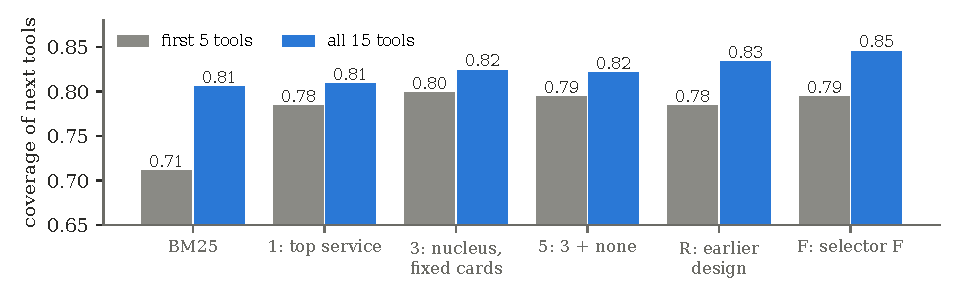
\includegraphics[width=\linewidth]{figures/fig_selector_heldout.pdf}
\caption{Held-out check on 500 agent searches from a different batch: share of the next tools covered by the first 5
and by all 15 returned tools. Variant numbers as in Table~\ref{tab:study}; R is the earlier recommendations design of
App.~\ref{app:rec}. The vertical axis starts at 0.65.}
\label{fig:heldout}
\end{figure}

\subsection{Offline: DM against shipped mechanisms and an LLM router}\label{sec:retrieval}
On the 120 hand-written queries, a server-then-tool DM hierarchy, the first version of our selector, ranked better
than every shipped mechanism and an LLM router that reads one line per tool (Table~\ref{tab:retrieval}). At 613 tools
it put the right tool first for 93\% of queries, against 48--54\% for the Claude Code-style, BM25 and embedding
mechanisms and 86\% for the router, which cost three times as much per query and took 2.4 times as long. Adding 463
decoy-rich tools lowered hit@1 by 3--6 points for every mechanism and left the order unchanged. General-purpose
embeddings did poorly, as ToolRet found~\citep{shi2025toolret}. On 183 queries written by agents in live runs the gap
was smaller: hit@1 0.60 for the DM against 0.45 for BM25, and hit@5 0.70 against 0.66, because agents write
keyword-style queries that suit lexical search.

\begin{table}[t]
\centering\small
\caption{Offline retrieval on 120 hand-written queries. Hit@$k$: a right tool is among the first $k$. Cost per
1{,}000 queries and median latency of the selecting call at 613 tools; name, BM25 and embedding search run locally.
Bold: best per accuracy column.}
\label{tab:retrieval}
\setlength{\tabcolsep}{5pt}
\begin{tabular}{@{}lcccccc@{}}
\toprule
& \multicolumn{2}{c}{613 tools} & \multicolumn{2}{c}{1{,}076 tools} & & \\
\cmidrule(lr){2-3}\cmidrule(lr){4-5}
Mechanism & hit@1 & hit@5 & hit@1 & hit@5 & \$/1k queries & latency, s \\
\midrule
Claude Code style & 0.48 & 0.71 & 0.45 & 0.65 & 0 & 0.01 \\
BM25 & 0.54 & 0.75 & 0.49 & 0.76 & 0 & $<$0.01 \\
embeddings & 0.51 & 0.80 & 0.47 & 0.75 & $\approx$0 & 0.67 \\
LLM router & 0.86 & \textbf{0.98} & 0.82 & \textbf{0.98} & 0.44 & 1.31 \\
DM hierarchy & \textbf{0.93} & 0.97 & \textbf{0.88} & 0.97 & 0.15 & 0.54 \\
\bottomrule
\end{tabular}
\end{table}

\subsection{Main test: DeepSeek V4.1 Flash, 15 repeats}\label{sec:main}
Each of the 37 tasks ran 15 times under BM25 and under \F{}, 555 slots and 1{,}110 runs. Selector~F used fewer tokens:
0.874$\times$ [0.82, 0.93], $p=0.0002$, a 12.6\% reduction, with fewer tokens on 361 of 555 slots
(Table~\ref{tab:deepseek}, Figure~\ref{fig:tokens}). Agents made 3.9 fewer searches per run, 7.1 against 11.1, made
8\% fewer LLM calls and sent 5\% smaller prompts per call. They read 1.3 more full definitions per run with
\texttt{tool\_describe}, which cost far less than the searches saved. Pass rates were equal, 550 of 555 each, with 5
discordant slots each way. Wall time did not change: the DM's second per search was offset by fewer turns. Cost per
run rose by 20\%, 1.20$\times$ [1.13, 1.28], because the DM fee of \$0.0025 per run is large next to an agent that
costs under a cent per run; \S\ref{sec:cost} discusses this. The saving was largest on the 7 multi-service tasks,
0.76$\times$, against 0.88$\times$ on the 22 single-service tasks.

\begin{table}[t]
\centering\footnotesize
\caption{Main test with DeepSeek V4.1 Flash: 37 tasks, 15 repeats, 555 same-time pairs. Per-run metrics as mean /
median. Ratio: geometric mean of per-slot ratios of \F{} to BM25, averaged per task, with a task-level bootstrap 95\%
CI; $p$: $t$-test over the 37 task means; for searches, the paired difference per run. Cost includes the DM fee.
Bold: the better value where the difference is significant.}
\label{tab:deepseek}
\setlength{\tabcolsep}{4pt}
\begin{tabular}{@{}lccll@{}}
\toprule
Metric & BM25 & \F{} & \F{} vs BM25 [95\% CI] & $p$ \\
\midrule
Passed runs & 550/555 & 550/555 & 5 vs 5 discordant & 1.00 \\
Tokens per run & 791k / 553k & \textbf{680k / 507k} & 0.874$\times$ [0.82, 0.93] & 0.0002 \\
LLM calls per run & 29.0 / 26 & \textbf{26.8 / 24} & 0.92$\times$ [0.88, 0.96] & 0.0007 \\
Searches per run & 11.1 / 10 & \textbf{7.1 / 6} & $-$3.9 [$-$5.0, $-$3.0] & $<$0.0001 \\
Prompt tokens per call, median & 21.1k & \textbf{20.1k} & 0.95$\times$ [0.93, 0.98] & 0.0006 \\
Cost per run, \$ & \textbf{0.0082 / 0.0068} & 0.0100 / 0.0089 & 1.20$\times$ [1.13, 1.28] & $<$0.0001 \\
Wall time per run, s & 137 / 120 & 140 / 120 & 1.01$\times$ [0.96, 1.07] & 0.75 \\
\bottomrule
\end{tabular}
\end{table}

\begin{figure}[t]
\centering
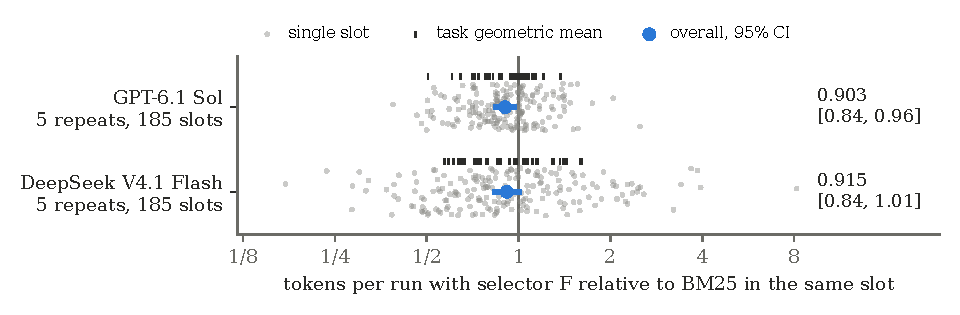
\includegraphics[width=\linewidth]{figures/fig_tokens.pdf}
\caption{Tokens per run with \F{} relative to BM25 in the same slot. Grey: single slots; black ticks: the 37
task-level geometric means; blue: overall geometric mean of the task means with a task-level bootstrap 95\% CI.
With DeepSeek, single slots range from 0.12 to 8.2, so only paired averages over many slots are informative.}
\label{fig:tokens}
\end{figure}

\subsection{Second agent model: GPT-6.1 Sol, 5 repeats}\label{sec:sol}
The same design with GPT-6.1 Sol and 5 repeats, 185 slots, also showed fewer tokens: 0.903$\times$ [0.84, 0.96],
$p=0.004$, a 9.7\% reduction (Table~\ref{tab:sol}). Sol searched less than DeepSeek to begin with, 5.5 times per run
with BM25, and 2.2 times with \F{}, 60\% fewer. It made 12\% fewer LLM calls, its prompts per call did not change,
and pass rates were equal, 172 and 173 of 185. Cost did not change, 0.99$\times$ [0.95, 1.03], since Sol's fee per run
was small next to its LLM cost and since cache writes, which \F{} does not reduce, made up more than half of that cost.

For comparison at equal size, the plan fixed in advance a random draw of 5 of the 15 DeepSeek repeats per task. On
that subsample the reduction was 0.915$\times$ [0.84, 1.01], $p=0.07$: similar in size but not significant, as the
power estimate for DeepSeek's higher noise predicted. The full 15-repeat result remains DeepSeek's verdict.

\begin{table}[t]
\centering\scriptsize
\caption{GPT-6.1 Sol, 37 tasks, 5 repeats, 185 same-time pairs, next to the pre-specified DeepSeek subsample of 5 of
15 repeats per task, also 185 pairs. Per-run metrics as mean / median; ratios and $p$ as in Table~\ref{tab:deepseek}.
Cost includes cache writes and the DM fee. Bold: the better value where the difference is significant.}
\label{tab:sol}
\setlength{\tabcolsep}{3pt}
\begin{tabular}{@{}lccll ll@{}}
\toprule
& \multicolumn{4}{c}{GPT-6.1 Sol} & \multicolumn{2}{c}{DeepSeek, 5 of 15 repeats} \\
\cmidrule(lr){2-5}\cmidrule(lr){6-7}
Metric & BM25 & \F{} & \F{} vs BM25 & $p$ & \F{} vs BM25 & $p$ \\
\midrule
Passed runs & 172/185 & 173/185 & 4 vs 5 discordant & 1.00 & 184 vs 182 passed & 0.63 \\
Tokens per run & 193k / 168k & \textbf{171k / 133k} & 0.903$\times$ [0.84, 0.96] & 0.004 & 0.915$\times$ [0.84, 1.01] & 0.07 \\
LLM calls per run & 13.4 / 13 & \textbf{11.5 / 10} & 0.88$\times$ [0.83, 0.92] & $<$0.0001 & 0.95$\times$ [0.89, 1.01] & 0.07 \\
Searches per run & 5.5 / 5 & \textbf{2.2 / 2} & $-$3.3 [$-$4.5, $-$2.2] & $<$0.0001 & $-$3.4 [$-$4.5, $-$2.4] & $<$0.0001 \\
Cost per run, \$ & 0.0724 / 0.0641 & 0.0715 / 0.0630 & 0.99$\times$ [0.95, 1.03] & 0.63 & 1.25$\times$ [1.15, 1.36] & $<$0.0001 \\
Wall time per run, s & 53 / 45 & 52 / 41 & 0.99$\times$ [0.92, 1.05] & 0.69 & 1.04$\times$ [0.95, 1.14] & 0.38 \\
\bottomrule
\end{tabular}
\end{table}

\subsection{Failure analysis: the Git family}\label{sec:failures}
An earlier design, which took only the top service and lacked the fixed cards, failed \texttt{gh\_open\_pr} in 3 of
15 runs while BM25 passed all 15 (App.~\ref{app:rec}). We asked the DM's service question for every distinct query
from that batch that names exactly one service, 2{,}477 queries. The DM chose the named service for 97.9\%. Of its 51
errors, 47 were within Git, GitHub and GitLab, most often Git for a GitHub query, and in 45 the named service came
second. By service it chose correctly 608 of 639 times for GitHub, 86 of 95 for Git and 325 of 332 for GitLab, and in
every case for Atlassian, Sentry, Slack, Notion, CloudWatch, MongoDB, Postgres and EKS. The errors came from the
service cards, which did not say that pull requests and branches live on GitHub rather than in the local Git copy.
With the fixed cards and the named-service rule, \F{} passed \texttt{gh\_open\_pr} in 15 of 15 runs. The remaining
failures are hard for both rankers: with Sol, \texttt{loki\_errors} and \texttt{prom\_threshold} account for 8 of
BM25's 13 failures and 10 of \F{}'s 12; with DeepSeek, \texttt{prom\_threshold} failed 3 times under \F{} and 2 times
under BM25.

\subsection{Loading all tools: opencode}\label{sec:opencode}
Supporting runs with opencode on the 33 v1 tasks and 613 tools, two repeats per task and two inexpensive agent models,
show why harnesses search (Table~\ref{tab:opencode}). Without a catalog no tool task passed; with one, every
condition passed 96--100\% of runs. Loading every definition made the largest prompt about 182k tokens with DeepSeek;
with ranked search it was 12--16k, and the cost per run fell from \$0.072 to \$0.008--0.009, 8--9 times less. Pass
rate cannot separate the search mechanisms, which is why the main tests compare tokens.

\begin{table}[t]
\centering\small
\caption{opencode on task set v1, 613 tools, two repeats per task. Pass: runs passed on the 25 tasks that need a
catalog tool. Largest prompt: median over those runs. Cost: mean LLM cost per run over all 33 tasks, without the
selector's fee. Bold: smallest largest prompt and lowest cost among conditions with catalog access.}
\label{tab:opencode}
\setlength{\tabcolsep}{4.5pt}
\begin{tabular}{@{}lcccccc@{}}
\toprule
& \multicolumn{3}{c}{DeepSeek V4.1 Flash} & \multicolumn{3}{c}{Tencent hy4} \\
\cmidrule(lr){2-4}\cmidrule(lr){5-7}
Condition & Pass & Largest prompt & \$/run & Pass & Largest prompt & \$/run \\
\midrule
no catalog & 0/25 & 9.6k & 0.0110 & 0/25 & 15.4k & 0.0154 \\
native & 25/25 & 181.9k & 0.0722 & 25/25 & 188.5k & 0.1039 \\
cc & 25/25 & 16.2k & 0.0089 & 25/25 & \textbf{32.0k} & \textbf{0.0375} \\
bm25 & 25/25 & 13.4k & 0.0093 & 25/25 & 33.6k & 0.0417 \\
groups & 25/25 & 29.0k & 0.0179 & 24/25 & 52.7k & 0.0562 \\
embed & 25/25 & 13.3k & 0.0090 & 23/25 & 49.0k & 0.0514 \\
llm & 25/25 & \textbf{11.7k} & \textbf{0.0076} & 25/25 & 32.6k & 0.0419 \\
dm & 25/25 & 14.0k & 0.0082 & 25/25 & 34.6k & 0.0470 \\
\bottomrule
\end{tabular}
\end{table}

\subsection{Cost by agent model}\label{sec:cost}
The DM fee is fixed per search; the saving scales with the agent model's price. Table~\ref{tab:cost} gives the two
measured results and prices the mean DeepSeek token mix at other models' list prices. With DeepSeek, \F{} cut the LLM
cost by 8.5\% before the fee, less than the token reduction because the tokens saved are mostly cached input, which
is cheap; the fee of \$0.0025 per run then made the mean run 22\% more expensive, or 20\% as the paired ratio of Table~\ref{tab:deepseek}. With Sol, the fee was \$0.0008
per run and cost was unchanged. If a model produced DeepSeek's token mix, \F{} would make runs 6--12\% more expensive
with inexpensive models and 7--9\% cheaper with mid-range and frontier ones, saving \$17--70 per 1{,}000 runs. Sol's
measured result is less favourable than this projection because its cost was dominated by cache writes, so the
projection is indicative only.

\begin{table}[t]
\centering\footnotesize
\caption{LLM cost per run with BM25 and with \F{}, DM fee included. Measured: the main tests, mean per run. Projected:
the mean DeepSeek token mix per run, 27.5k uncached input, 755.9k cached input and 11.1k output tokens with BM25 and
24.8k, 648.4k and 10.8k with \F{}, priced at list prices in \$ per million tokens, plus the measured fee of \$0.0025 per
run. $^{a}$Also includes cache writes at \$2.50 per million tokens.}
\label{tab:cost}
\setlength{\tabcolsep}{4pt}
\begin{tabular}{@{}llcccr@{}}
\toprule
& Agent model & Price, in / cached / out & BM25 \$/run & \F{} \$/run & Change \\
\midrule
\multirow{2}{*}{Measured} & DeepSeek V4.1 Flash, DeepInfra & 0.098 / 0.003 / 0.29 & \textbf{0.0082} & 0.0100 & +22\% \\
& GPT-6.1 Sol$^{a}$ & 2.00 / 0.10 / 10.00 & 0.0724 & 0.0715 & $-$1\% \\
\midrule
\multirow{5}{*}{Projected} & DeepSeek V4.1 Flash, list price & 0.15 / 0.003 / 0.60 & \textbf{0.0131} & 0.0147 & +12\% \\
& Claude Haiku 5.5 & 0.10 / 0.01 / 0.50 & \textbf{0.0159} & 0.0169 & +6\% \\
& Claude Sonnet 5.5, GPT-6.1 Sol & 2.00 / 0.10 / 10.00 & 0.2420 & \textbf{0.2247} & $-$7\% \\
& Kimi K3.1 Pro & 2.00 / 0.20 / 10.00 & 0.3176 & \textbf{0.2895} & $-$9\% \\
& Claude Fable 5.1 & 10.00 / 0.25 / 50.00 & 1.0211 & \textbf{0.9510} & $-$7\% \\
\bottomrule
\end{tabular}
\end{table}

%=====================================================================
\section{Discussion}\label{sec:discussion}
%=====================================================================
\paragraph{Fewer searches matter more than cheaper searches.} A search costs the agent a full turn: the model re-reads
its whole context to write the query and again to read the answer. Selector~F cut searches by 36\% with DeepSeek and 60\%
with Sol; the tokens saved came from fewer LLM calls, not from shorter answers, since \F{}'s answers are longer than
BM25's. A better first answer, with the right service's likely next tools listed by name, saves the turns that a
rephrased query would cost.

\paragraph{When the DM pays off.} The fee is fixed per search, while the saving is a share of the agent's own cost.
The DM therefore pays off with expensive agent models, many tools and search-heavy work, and does not with inexpensive
models such as DeepSeek V4.1 Flash, whose whole run costs about a cent. An efficient agent that searches little, like
Sol, gains fewer searches to remove, and where cache writes dominate cost, as with Sol, fewer cached reads save
little.

\paragraph{What ``universal'' means here.} Selector~F needs one API call per question, no training, and only the query
and the catalog; it worked unchanged with two agent models and slots into any harness that has a search tool. We have
not shown that it helps in every harness, catalog or kind of task.

\paragraph{What the DM is good and bad at.} The DM is good at comparing options: choosing a service among cards or a
tool among a service's tools. It is poor at judging a tool in isolation, as the yes/no variants showed, and at
predicting the next step of an agent, where always choosing the shell did better (App.~\ref{app:session}). Its
answers depend on the option texts: the Git-family errors came from service cards, not from the model.

%=====================================================================
\section{Threats to validity}\label{sec:threats}
%=====================================================================
\paragraph{Scope.} The services are simulated: real services return longer and messier results, which would raise
token counts and could change how agents search. The tasks are coding tasks only. Two agent models were tested, and
the main tests used one harness, Hermes Agent; opencode results come from an earlier selector and task set.

\paragraph{Design choices made before the tests.} Selector~F was designed in exploratory runs on a separate long task and in
the offline study, before the main tests; we checked it on held-out searches from a different batch. The usage lists
come from the same task suite but are built leave-one-task-out. The connected-services note in every prompt may raise
search rates above those of an unprompted agent; it is the same for both conditions.

\paragraph{Exclusions and interruptions.} \texttt{k8s\_crashloop} was excluded for both conditions, as stated in each
plan. Interim looks, container restarts and reruns after rate-limit errors are logged in the plans
(App.~\ref{app:plans}); no run was dropped for its result.

\paragraph{Drift and baselines.} Our A/A comparison could not rule out drift of the size we measure, so only
same-time pairs support the claims; the earlier six-ranker comparison of App.~\ref{app:sixrank} does not meet this
standard. The baseline is Hermes Agent's BM25 as shipped; a tuned BM25 or query rewriting might narrow the gap.

%=====================================================================
\section{Related work}\label{sec:related}
%=====================================================================
\paragraph{Tool retrieval for large catalogs.} Retrieving tools before generation is the standard answer to large
catalogs~\citep{qin2023toolllm,oats2026}. AnyTool~\citep{du2024anytool} selects among over 16{,}000 APIs with a
hierarchy of LLM agents, category first and tool second, and MCP-Zero~\citep{fei2025mcpzero} brings the
server-then-tool idea to MCP; \F{} applies the same hierarchy with a decision model instead of an LLM.
RAG-MCP~\citep{gan2025ragmcp} retrieves MCP tool descriptions with embeddings to reduce prompt bloat, and
\citet{mudunuri2026semantic} select among 121 tools of five MCP servers with embeddings, without agent runs. ToolRet
finds that general-purpose embedding retrievers do poorly on tool retrieval~\citep{shi2025toolret}, and
\citet{selection2026retrieval} find that selecting a tool is largely retrieval. Agent skills~\citep{anthropic2025skills}
apply progressive disclosure to instructions; our service cards and handbook play this role for the catalog.

\paragraph{MCP benchmarks.} LiveMCPBench~\citep{mo2025livemcpbench}, MCPMark~\citep{wu2025mcpmark},
MCP-Atlas~\citep{mcpatlas2026} and Toolathlon~\citep{toolathlon2025} score agents' task completion with real MCP
tools. We fix the agent, vary only the selector, and simulate back ends so that runs are reproducible and writes can
be graded safely.

\paragraph{Vendor reports.} Stacklok compared its MCP Optimizer with Anthropic's tool search on 2{,}792
tools~\citep{stacklok2025optimizer}, and Arcade tested Anthropic's tool search on about 4{,}000
tools~\citep{arcade2025toolsearch}. Both measure selection accuracy, not task completion or tokens per task.

\paragraph{Decision models.} The Artificial Analysis Decision Index~\citep{aa2026decisionindex} and an analysis of
it~\citep{olson2026decision} compare DMs with LLMs on standalone decisions, including tool calling. We place a DM
inside agents as the tool selector and measure its effect on whole runs.

%=====================================================================
\section{Conclusion}\label{sec:conclusion}
%=====================================================================
A decision model can serve as an agent's tool selector. Built on \msd{}, \F{} chooses services with a ``none'' option,
then asks two questions per service and adds usage-based names, at about three DM calls per search. Offline it put
the right tool first for 92\% of hand-written queries at 1{,}076 tools, against 49\% for BM25. Inside Hermes Agent, in
pre-planned same-time paired tests, it used 12.6\% fewer tokens than BM25 with DeepSeek V4.1 Flash and 9.7\% fewer
with GPT-6.1 Sol, with 36--60\% fewer searches and equal pass rates. Its fee made runs 20\% more expensive with the
inexpensive model and left cost unchanged with the frontier model; the saving grows with the agent model's price and
with how much it searches. These results hold for coding agents with simulated services, two agent models and one
harness; testing other harnesses, real services and non-coding work is the next step.

\paragraph{Reproducibility.} We will release the tool harvester, catalog snapshots, simulator, tasks with hidden tests
and reference solutions, the selector and ranking server, the Hermes patch, the sandbox setup, all run records, the
analysis plans and the analysis and figure scripts.

\bibliographystyle{plainnat}
\bibliography{references}

\appendix
%=====================================================================
\section{Sandbox hardening}\label{app:hardening}
%=====================================================================
The isolation of \S\ref{sec:setup} is the result of fixes made during development; runs made before them are not
reported. In order:
\begin{itemize}
\item Agents run as an unprivileged user with an empty environment and no credentials; experiment files are readable
only by root and the API key is held by a local proxy that admits only the experiment models, because harness-level
permissions alone let an agent read hidden tests through absolute paths.
\item Each Hermes run gets its own mount namespace with a private work directory, home directory and \texttt{/tmp}, so
runs cannot see each other's files or leftovers.
\item The MCP server accepts only requests that carry a per-run token the agent's shell cannot read, so the shell cannot
list the catalog or query the ranker directly.
\item Hermes's deny list blocks probing commands: \texttt{curl}, \texttt{wget}, \texttt{ps}, \texttt{ss},
\texttt{netstat}, \texttt{nmap}, \texttt{lsof}, \texttt{/proc}, \texttt{localhost} and \texttt{find /}.
\item Rankers are compared inside Hermes's own bridge rather than through a separate search tool with a generic call
tool, so that only the ranking differs.
\item The provider and sampling are pinned as described in \S\ref{sec:setup}.
\end{itemize}

%=====================================================================
\section{Tool catalog and task set}\label{app:catalog}
%=====================================================================
{\centering\footnotesize
\captionof{table}{The real tool catalog: tools per MCP server, from each server's own \texttt{tools/list}.}
\label{tab:catalog}
\setlength{\tabcolsep}{3.5pt}
\begin{tabularx}{\linewidth}{@{}l X r@{}}
\toprule
Catalog & Servers with their numbers of tools & Tools \\
\midrule
main & Linear 198, Atlassian 98, GitHub 91, Grafana 81, Git 28, MongoDB 27, Playwright 25, Notion 24, Kubernetes 23,
Sentry 9, Slack 8, Postgres 1 & 613 \\
extra & GitLab 127, monday 84, Salesforce 74, Heroku 33, HubSpot 21, AWS CloudWatch 19, AWS EKS 16, Airtable 16,
Filesystem 14, CircleCI 13, Browserbase 9, Memory 9, Netlify 9, Terraform 9, Elasticsearch 4, ClickHouse 3, Figma 2,
Docker 1 & +463 \\
\midrule
all & 30 servers & 1{,}076 \\
\bottomrule
\end{tabularx}
\par}
\bigskip
{\small
\begin{longtable}{@{}>{\raggedright\arraybackslash}p{1.4cm}>{\raggedright\arraybackslash}p{2.6cm}>{\raggedright\arraybackslash}p{7.1cm}>{\raggedright\arraybackslash}p{2.4cm}@{}}
\caption{Task set v2, 38 tasks. Prompts are shortened to their first sentence and shown without the escape clause. Services: the servers of the needed tools, in order; $+w$: number of required writes; $\star$: new in v2.}\label{tab:tasks_v2}\\
\toprule Category & Task & First sentence of prompt & Services \\ \midrule\endfirsthead
\toprule Category & Task & First sentence of prompt & Services \\ \midrule\endhead
control & \texttt{c\_chunk} & chunk in batching/chunk.py drops the last partial chunk. & -- \\
control & \texttt{c\_dedupe} & dedupe in collections\_util/dedupe.py loses the original order. & -- \\
control & \texttt{c\_duration} & parse\_duration in timeutil/duration.py only understands hours. & -- \\
control & \texttt{c\_leap} & is\_leap in calendar\_util/leap.py is wrong for some years. & -- \\
single & \texttt{confluence\_limits} & Our public API rate limits changed. & atlassian \\
single & \texttt{eks\_importer} $\star$ & The data team's nightly batch-importer job has failed three nights in a row. & aws\_eks \\
single & \texttt{gh\_ci\_fail} & Pull request \#214 in acme/payments can't be merged because a check is red. & github $+1w$ \\
single & \texttt{gh\_codesearch} & SUPPORTED\_CURRENCIES in shop/currencies.py has drifted from the company-wide canonical list, which lives in another repository. & github \\
single & \texttt{gh\_dependabot} & Security says acme/payments has dependencies with known vulnerabilities. & github \\
single & \texttt{gh\_issue} & Please implement acme/payments\#301. & github \\
single & \texttt{gh\_open\_pr} & Pagination in acme/catalog is broken (see \#57). & github $+2w$ \\
single & \texttt{gh\_release} & We are behind on the ledger API. & github \\
single & \texttt{gh\_review} & There is reviewer feedback waiting on pull request \#88 in acme/ledger. & github $+1w$ \\
single & \texttt{grafana\_incident} & We are in the middle of an incident about checkout timeouts and the responders agreed on a mitigation. & grafana $+1w$ \\
single & \texttt{jira\_impl} & Pick up PAY-412: implement it, then move it to review. & atlassian $+1w$ \\
single & \texttt{k8s\_crashloop} & ledger-worker keeps restarting in production (namespace ledger) since the last config change. & kubernetes \\
single & \texttt{k8s\_oom} & report-builder (namespace reports) keeps dying in production. & kubernetes \\
single & \texttt{linear\_bug} & Fix ENG-77 and move it to In Review. & linear $+1w$ \\
single & \texttt{loki\_errors} & Customers stopped getting shipping e-mails at around 06:00 UTC today; the notifier service is the suspect. & grafana \\
single & \texttt{mongo\_shape} & The nightly export has started crashing on recent orders. & mongodb \\
single & \texttt{notion\_runbook} & We are rotating the webhook signing keys. & notion \\
single & \texttt{oncall\_contact} & Set ESCALATION\_CONTACT in ops/escalation.py to the e-mail address of whoever is on call for the payments team right now. & grafana \\
single & \texttt{pg\_migration} & Add migrations/0042\_payments\_merchant\_idx.sql with an index named payments\_merchant\_created\_idx for looking up a merchant's payments by creation time. & postgres \\
single & \texttt{prom\_threshold} & Set SLOW\_REQUEST\_MS in alerts/config.py to twice the checkout service's current p99 request latency, in milliseconds. & grafana \\
single & \texttt{sentry\_events} & Since this morning's deploy some clients get HTTP 500 from POST /refunds. & sentry \\
single & \texttt{sentry\_fix} & The noisiest production error of payments-api right now needs to go. & sentry $+1w$ \\
single & \texttt{slack\_decision} & The payments team agreed on a new webhook retry policy in a chat discussion. & slack $+1w$ \\
multi & \texttt{cw\_reports} $\star$ & The legacy reports API has been answering 502 since yesterday evening. & aws\_cloudwatch, slack $+1w$ \\
multi & \texttt{gl\_pipeline} $\star$ & The main-branch pipeline of billing-legacy is red. & gitlab $+1w$ \\
multi & \texttt{linear\_notion\_pr} $\star$ & Do ENG-91 the way our API guidelines say, and open a pull request for it from a branch named eng-91 against main in acme/public-api. & linear, notion, github $+1w$ \\
multi & \texttt{multi\_alert} & Something is paging for the checkout service. & grafana, slack $+1w$ \\
multi & \texttt{multi\_jira\_conf} & Implement PAY-530 as its design document specifies, then leave a one-line summary on the ticket. & atlassian $+1w$ \\
multi & \texttt{multi\_sentry\_gh} & A recent change to ledger-worker introduced a reconciliation bug that shows up as a production error. & sentry, github $+1w$ \\
multi & \texttt{promo\_sentry\_jira} $\star$ & Android users report they can't apply promo codes. & sentry, atlassian $+1w$ \\
absent & \texttt{absent\_jira} & Implement PAY-999 in payments/limits.py. & -- \\
absent & \texttt{absent\_release} & Pin SDK\_VERSION in sdk/version.py to the newest release of acme/ghost-sdk (without the leading v). & -- \\
absent & \texttt{absent\_sentry} & The billing-cron error someone mentioned in standup needs fixing in billing/cron.py. & -- \\
absent & \texttt{absent\_slack} & Set CACHE\_TTL\_S in cache/config.py to the value the platform team agreed on. & -- \\
\bottomrule
\end{longtable}

}

%=====================================================================
\section{Analysis plans and interim-look logs}\label{app:plans}
%=====================================================================
The three plans below are reproduced verbatim, including their interim-look logs, as they stood when each batch's
final analysis was run. File and condition names refer to the run records: \texttt{hermes\_default} is BM25,
\texttt{hermes\_dmfrankenbridge} is \F{} and \texttt{hermes\_dmrec510bridge} is the recommendations design of
App.~\ref{app:rec}. The first plan was written after an interim look, which it records; the other two were written
before their first run.

\fvset{fontsize=\fontsize{6.6}{7.9}\selectfont, breaklines=true, breakanywhere=true, frame=single, framesep=1.5mm}
\subsection*{C.1 Recommendations design with DeepSeek V4.1 Flash}
\VerbatimInput{plans/plan_rec510.md}
\subsection*{C.2 Selector~F with DeepSeek V4.1 Flash}
\VerbatimInput{plans/plan_franken.md}
\subsection*{C.3 Selector~F with GPT-6.1 Sol}
\VerbatimInput{plans/plan_franken_sol.md}

%=====================================================================
\section{An earlier design: recommendations}\label{app:rec}
%=====================================================================
Before \F{} we tested a recommendations design under the same protocol: only the top service, with the original
cards; its five best tools with one-line descriptions; and up to ten names from the DM's next-best tools and the
service's most-used tools. With DeepSeek V4.1 Flash, 37 tasks and 15 repeats, 555 same-time pairs, it used
0.910$\times$ the tokens of BM25 [0.85, 0.97], $p=0.009$, a second, independent confirmation of a token reduction
with a DM selector. Searches fell from 11.5 to 7.4 per run and LLM calls by 6\%, 0.94$\times$ [0.90, 0.98]. Cost per
run rose by 8.5\%, 1.085$\times$ [1.02, 1.16], and wall time did not change, 1.04$\times$ [0.97, 1.11]. It passed 549
runs against 552 for BM25, with 6 and 3 discordant slots, McNemar $p=0.51$; three of its failures were
\texttt{gh\_open\_pr}, which led to the analysis of \S\ref{sec:failures}. Its 400 BM25-run searches are the agent set
of the offline study, and its BM25 runs the A/A comparison of \S\ref{sec:measuring}.

%=====================================================================
\section{The six-ranker comparison of the first version}\label{app:sixrank}
%=====================================================================
The first version of this paper compared six rankers inside Hermes Agent's bridge with DeepSeek V4.1 Flash on all
38 tasks, three repeats each, 114 runs per ranker (Table~\ref{tab:sixrank}). Two caveats apply. Three repeats give too
few pairs for effects of 10\%, and only BM25, DM and random ran back to back in each slot, while the other three ran
later in separate batches, so their differences from BM25 are within the drift we later measured
(\S\ref{sec:measuring}). The robust finding is that ranking matters: random ranking used 1.57$\times$ the tokens of
BM25. All rankers, random included, passed 96.5--100\% of runs.

\begin{table}[ht]
\centering\small
\caption{Six rankers in Hermes Agent's bridge, first version: 38 tasks, three repeats, 114 runs per ranker. Tokens:
median per run. Ratio: geometric mean of per-slot token ratios against BM25 with a task-level bootstrap 95\% CI. LLM
calls and searches: mean per run. DM with ``none'' is the DM ranker with a ``none'' option. Not same-time for the last
three rows.}
\label{tab:sixrank}
\setlength{\tabcolsep}{5pt}
\begin{tabular}{@{}lccccc@{}}
\toprule
Ranker & pass@1 & Tokens & Ratio [95\% CI] & LLM calls & Searches \\
\midrule
BM25 & 0.991 & 558k & -- & 29.0 & 11.4 \\
DM & 0.991 & 480k & 0.93 [0.82, 1.04] & 27.9 & 9.7 \\
random & 1.000 & 1{,}051k & 1.57 [1.38, 1.79] & 34.9 & 12.8 \\
DM with ``none'' & 0.991 & 459k & 0.88 [0.78, 0.98] & 27.4 & 10.1 \\
embeddings & 0.965 & 562k & 0.91 [0.81, 1.03] & 27.9 & 11.1 \\
Claude Code style & 0.991 & 576k & 1.02 [0.89, 1.16] & 23.2 & 6.0 \\
\bottomrule
\end{tabular}
\end{table}

%=====================================================================
\section{Next-tool prediction in a real session}\label{app:session}
%=====================================================================
This experiment motivates using the DM to select tools rather than to call them. We took the 395 tool decisions of one
real coding session and asked each model to predict the next tool among the 38 available. \msd{} reached an accuracy
of 0.49 and TypeSafe Jev~\citep{typesafejev} 0.60, both below always choosing the shell at 0.75, although the DMs'
top five contained the right tool 94--96\% of the time. In that session 51 always-loaded tool definitions took about
59k tokens, 93\% of the first request and 16\% of all context tokens read. Most tool choices in a coding session are
easy and the LLM must write every call's arguments; the DM is useful where the choice is hard, among hundreds of
rarely used catalog tools.

\end{document}
